\subsection{Interface}
    These are the commands that the web API will be using to maintain the database and receive commands.
    \begin{itemize}
        \item AddRecord
        \item Headers required:
        \begin{itemize}
            \item none
        \end{itemize}
        \item POST arguments:
        \begin{itemize}
            \item record : Record
        \end{itemize}
        \item Statuses:
        \begin{itemize}
        	\item 200 OK:
            \begin{itemize}
        		\item record ID : Integer
            \end{itemize}
        	\item 400 Bad Request
        	\item 500 Internal Server Error
        \end{itemize}

        \item RemoveRecord
        \item Headers required: 
        \begin{itemize}
        	\item Authorization
        \end{itemize}
        \item POST Arguments:
        \begin{itemize}
        	\item recordID : Integer
        \end{itemize}
        \item Statuses:
        \begin{itemize}
        	\item 200 OK : no data
        	\item 400 Bad Request
        	\item 401 Unauthorized
        	\item 500 Internal Server Error
        \end{itemize}

        \item ModifyRecord
        \item Headers required:
        \begin{itemize}
        	\item Authorization
        \end{itemize}
        \item POST Arguments:
        \begin{itemize}
        	\item recordID : Integer
        	\item record : Record
        \end{itemize}
        \item Statuses:
        \begin{itemize}
        	\item 200 OK : no data
        	\item 400 Bad Request
        	\item 401 Unauthorized
        	\item 500 Internal Server Error
        \end{itemize}


        \item GetRecord
        \item Headers required: 
        \begin{itemize}
            \item none
        \end{itemize}
        \item POST Arguments:
        \begin{itemize}
        	\item recordID : Integer
        \end{itemize}
        \item Statuses:
        \begin{itemize}
        	\item 200 OK :
            \begin{itemize}
                \item record : Record
            \end{itemize}
        	\item 400 Bad Request
        	\item 500 Internal Server Error
        \end{itemize}

        \item GetRecords
        \item Headers Required:
        \begin{itemize}
        	\item none
        \end{itemize}
        \item POST Arguments:
        \begin{itemize}
            \item maxResultCount : Integer
            \item resultStartOffset : Integer?
        	\item speciesFilter : String?
            \item abundanceFilter : Integer?
            \item userNameFilter : String?
            \item fullNameFilter : String?
            \item commentFilter : String?
            \item locationNameFilter : String?
            \item locationLatitudeProximityFilter : Float?
            \item locationLongitudeProximityFilter : Float?
            \item locationProximityRadius : Float?
        \end{itemize}
        \item Statuses: 
        \begin{itemize}
        	\item 200 OK : array of Record
        	\item 400 Bad Request
        	\item 500 Internal Server Error
        \end{itemize}

        \item AddResource
        \item Headers required: 
        \begin{itemize}
            \item none
        \end{itemize}
        \item POST Arguments:
        \begin{itemize}
        	\item resource : OctetStream
        \end{itemize}
        \item Statuses:
        \begin{itemize}
        	\item 200 OK :
            \begin{itemize}
        		\item resource ID : Integer
            \end{itemize}
        	\item 400 Bad Request
        	\item 500 Internal Server Error
        \end{itemize}

        \item GetResource
        \item Headers required:
        \begin{itemize}
            \item none
        \end{itemize}
        \item POST Arguments:
        \begin{itemize}
        	\item resourceID : Integer
        \end{itemize}
        \item Statuses:
        \begin{itemize}
        	\item 200 OK : 
            \begin{itemize}
                \item resource data : OctetStream
            \end{itemize}
        	\item 400 Bad Request
        	\item 500 Internal Server Error
        \end{itemize}
    \end{itemize}

\subsection{Detailed design}
    \subsubsection{Diagrams}
        \begin{figure}
            \centering
            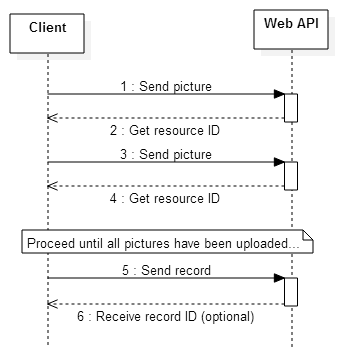
\includegraphics[scale=0.75]{server/working/SequenceDiagram-AddRecord.png}
            \caption{Sequence diagram: adding a record through the web API}
            \label{fig:addRecordSequenceDiagram}
        \end{figure}

        \begin{landscape}
            \begin{figure}
                \centering
                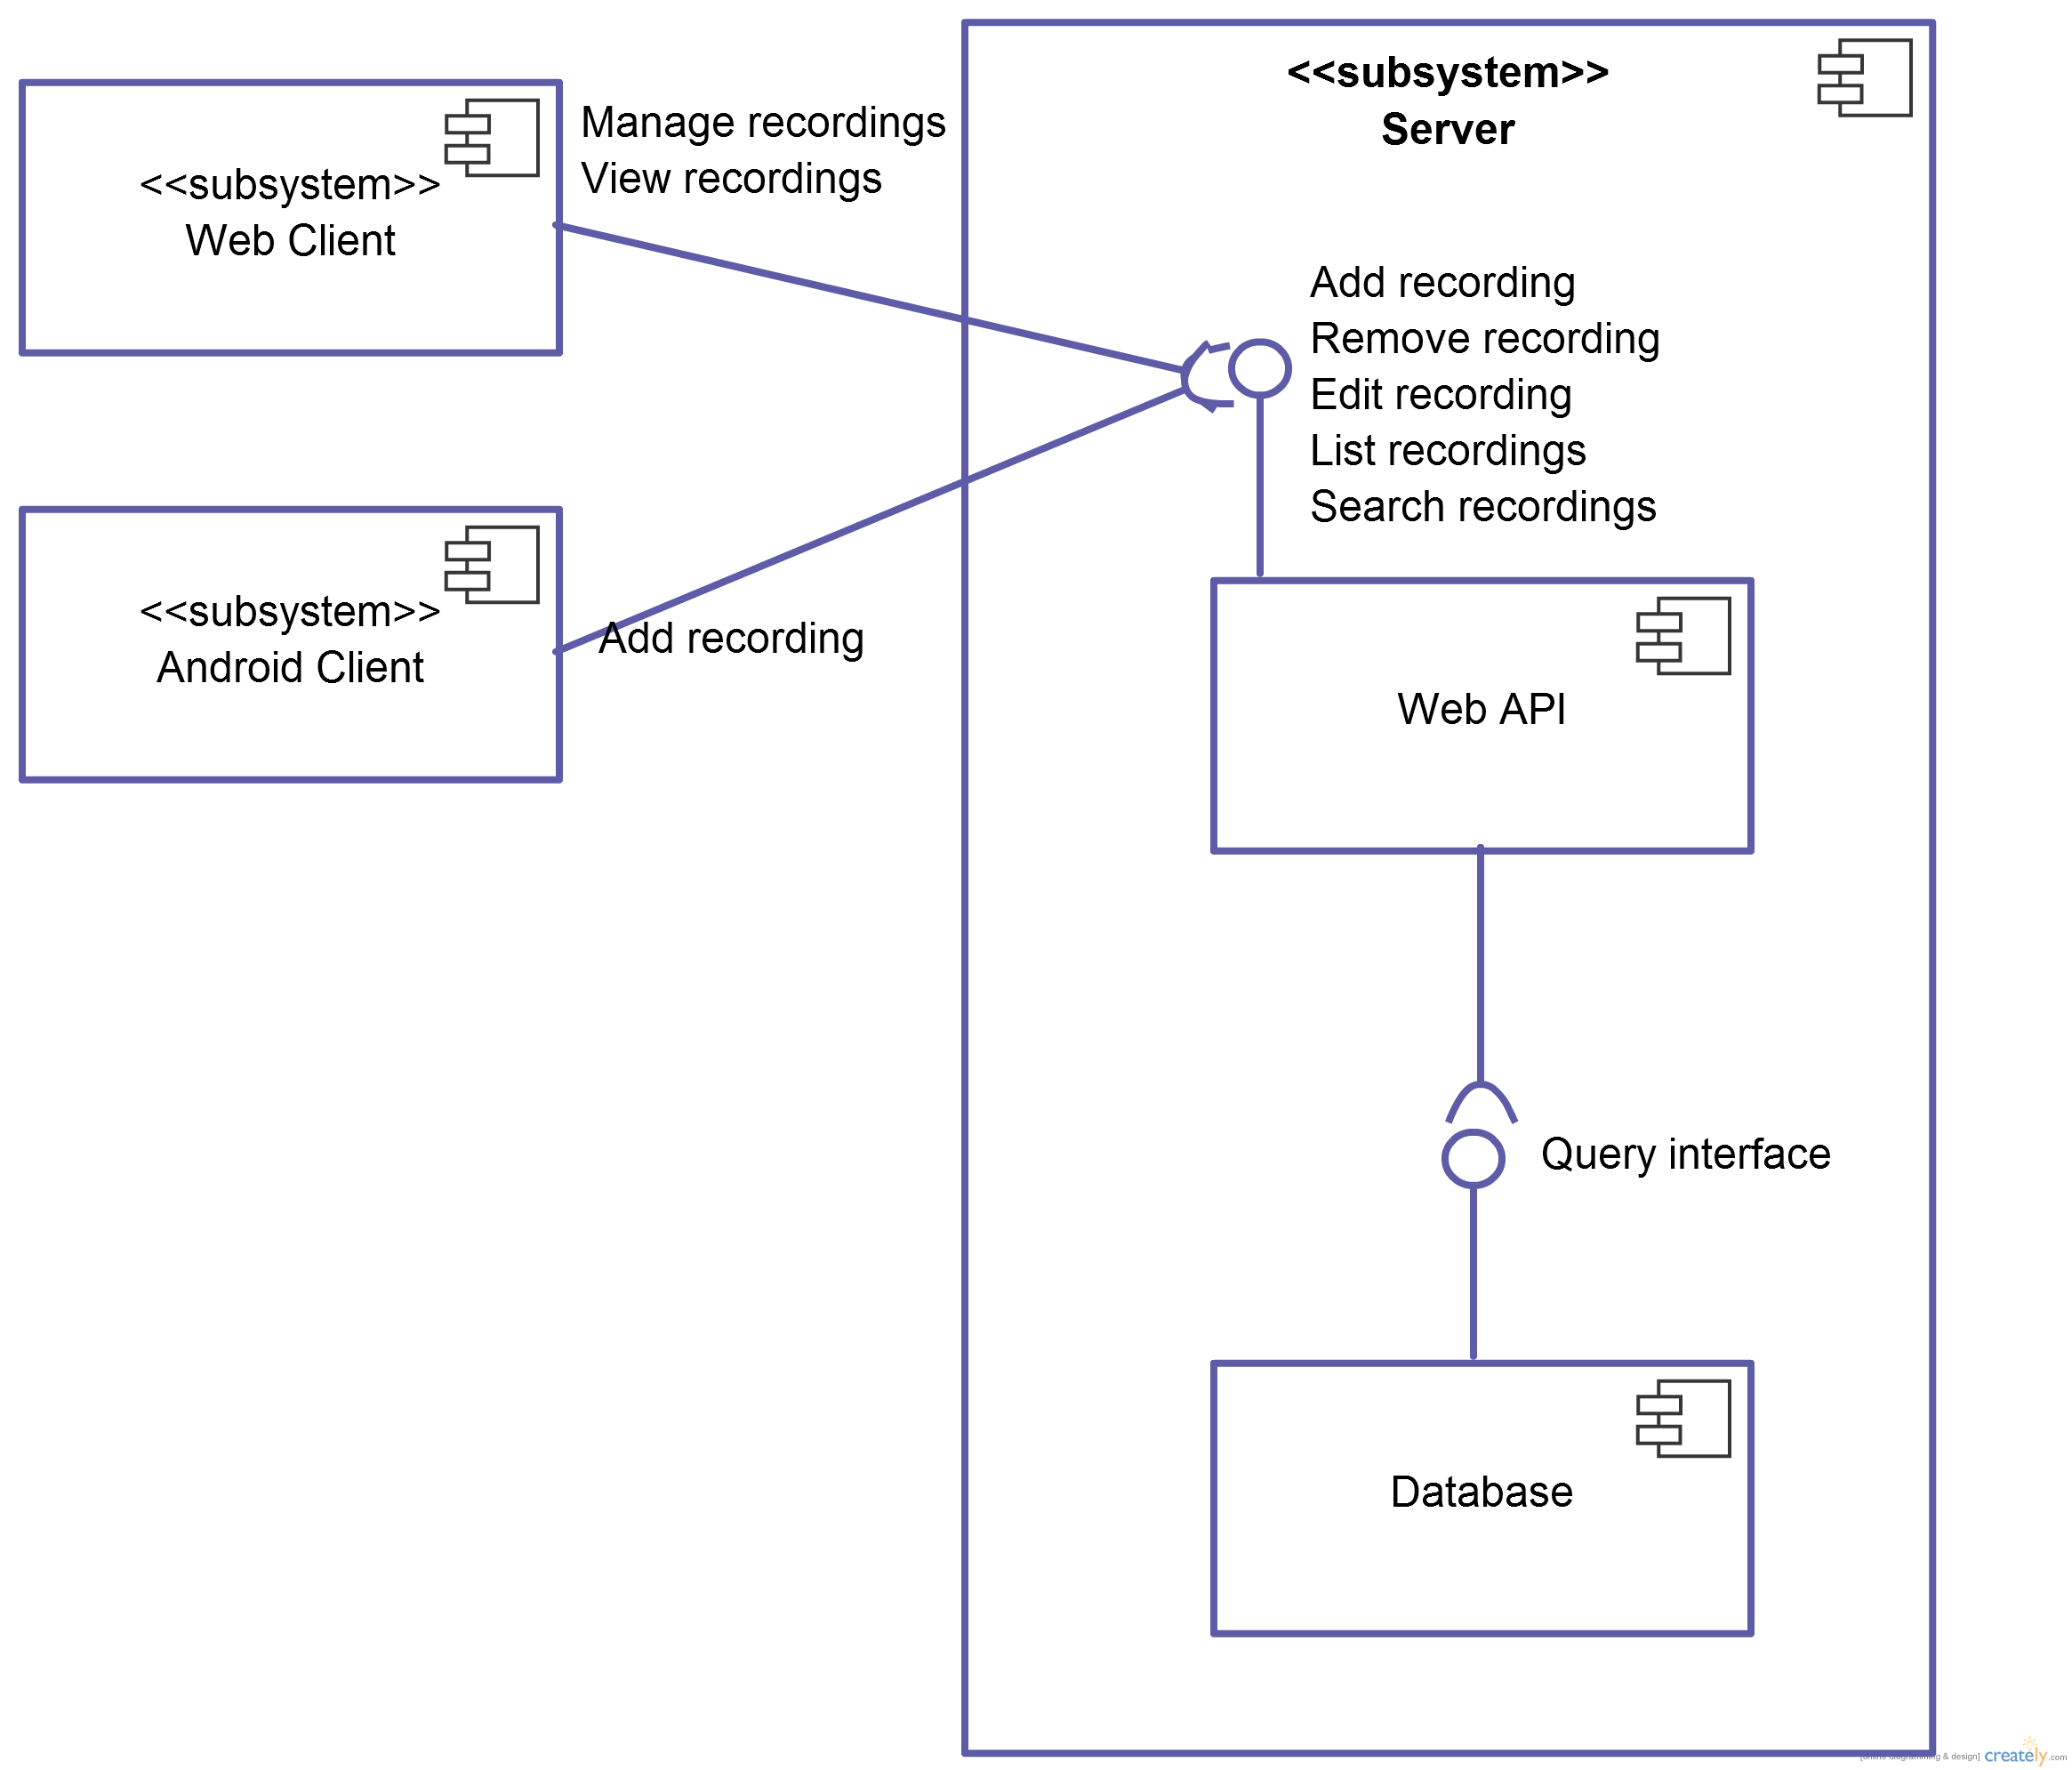
\includegraphics[scale=0.2]{server/ComponentDiagram.png}
                \caption{Web Api component Diagram}
                \label{fig:webAPIComponentDiagram}
            \end{figure}
        \end{landscape}

    \subsubsection{Significant data structures}

        The web API is going to make use of the Record and Specimen data structures, which will be exchanged between the server and its clients (the Android application and the website). They will be represented in a JSON format, which is readily available for use in PHP, JavaScript, and Android. Data types, where specified, are JSON data types. 

        The structure of a Record is as follows:
        \begin{itemize}
            \item Record : Object
            \begin{itemize}
                \item UserName : String
                \item UserPhone : String
                \item UserEmail : String
                \item LocationName : String 
                \item Timestamp : Number 
                \item LocationOS : String
                \item Specimens : Array of Specimen
            \end{itemize}
        \end{itemize}

        The structure of a Specimen is as follows:
        \begin{itemize}
            \item Specimen : Object
            \begin{itemize}
                \item SpeciesName : String
                \item LocationLatitude : Number
                \item LocationLongtitude : Number
                \item Abundance : Number
                \item Comment : String
                \item ScenePhoto : String (ID of a resource on the server)
                \item SpecimenPhoto : String (ID of a resource on the server)
            \end{itemize}
        \end{itemize}

        The web API is going to use a relational database as a data store.
        The database tables are as follows:

        \begin{itemize}
            \item Users
            \begin{itemize}
                \item UserId : INT auto-increment PK
                \item UserName : VARCHAR(20) not-null
                \item UserFullName : VARCHAR(50)
                \item UserPhone : VARCHAR(20)
                \item UserEmail : VARCHAR(50)
                \item UserPassword : BINARY(20)
            \end{itemize}
                
            \item Records
            \begin{itemize}
                \item RecordId : INT auto-increment PK
                \item UserId : INT not-null
                \item LocationName : VARCHAR(50)
                \item Timestamp : INT
                \item LocationOS : VARCHAR(10)
            \end{itemize}
                
            \item Resources
            \begin{itemize}
                \item ResourceId : INT auto-increment PK
            \end{itemize}

            \item Specimens
            \begin{itemize}
                \item SpecimenId : INT auto-increment PK
                \item RecordId : INT not-null
                \item SpeciesName : VARCHAR(255) not-null
                \item Latitude : FLOAT(10,6)
                \item Longitude : FLOAT(10,6)
                \item Abundance : INT
                \item Comment : TEXT
                \item ScenePhoto : INT
                \item SpecimenPhoto : INT   
            \end{itemize}
                \item Comment : String
                \item ScenePhoto : String (ID of a resource on the server)
                \item SpecimenPhoto : String (ID of a resource on the server)
            \end{itemize}
        \end{itemize}

        The web API is going to use a relational database as a data store.
        The database tables are as follows:

        \end{itemize}